\chapter{Program evaluation
 and review technique (PERT)}
This chapter is based on
Refs.\cite{ibook} and \cite{wiki-pert}.

PERT diagrams are 
used for scheduling a 
project consisting of a series
of interdependent activities
and estimating how
long it will take
to finish the project.
PERT diagrams were invented by the NAVY 
in 1958
to manage a submarine project.
Nowadays they are taught in many business 
and management courses.

A {\bf PERT diagram}
is a  Directed Acyclic Graph (DAG)
with the following properties. 
(See Fig.\ref{fig-pert-diag}
for an example of a PERT diagram).
The nodes $\rvE_i$ for $i=1, 2, \ldots, ne$ of a
PERT diagram are called {\bf events}.
 The edges $i\rarrow j$ of a PERT diagram are called
 {\bf activities}.
An event represents the starting 
(kickoff) date of one or more
activities.
A PERT diagram has a 
single root node ($i=1$, start event)
and a single leaf node ($i=ne$, end event).

The PERT diagram user 
must initially 
provide a
{\bf Duration Times (DT) table} which gives $(DO_{i\rarrow j}, 
DP_{i\rarrow j}, DM_{i\rarrow j})$ for each activity
$i\rarrow j$, where

$DO_{i\rarrow j}$= optimistic duration time 
of activity $i\rarrow j$

$DP_{i\rarrow j}$= pessimistic duration time 
of activity $i\rarrow j$

$DM_{i\rarrow j}$= median duration time 
of activity $i\rarrow j$

From the DT table, one calculates:

Duration time of activity $i\rarrow j$ 
\beq
D_{i\rarrow j}= \frac{1}{6}(DO_{i\rarrow j}+
DP_{i\rarrow j} +4DM_{i\rarrow j})
\eeq

Duration Variance of activity $i\rarrow j$
\beq
V_{i\rarrow j} = \left(
\frac{DO_{i\rarrow j}-DP_{i\rarrow j}} 
{DM_{i\rarrow j}}\right)^2
\eeq

Often,
it is convenient to define
\qt{dummy} edges with $D_{i\rarrow j}=0$.
That is perfectly fine.

Define:

$TES_i=$ Earliest start time for event $i$

$TLS_i=$ Latest start time for event $i$

$slack_i=TLS_i-TES_i=$ slack for event $i$

$TEF_{i\rarrow j}=TES_i + D_{i\rarrow j}=$ 
Earliest finish 
time for activity $i\rarrow j$.

$TLF_{i\rarrow j}=TLS_j-D_{i\rarrow j}=$ 
 Latest finish 
time for activity $i\rarrow j$. See footnote below.
\footnote{
In the popular educational literature,
the edge variables
$TEF_{i\rarrow j}$
and $TLF_{i\rarrow j}$
are sometimes associated 
 with
the nodes, but they 
are clearly edge variables.
This makes things confusing.
The reason this is done is
that some software draws PERT diagrams as
trees whereas other software
draws them as DAGs. For trees,
storing $TEF_{i\rarrow j}$
and $TLF_{i\rarrow j}$ in a node
makes some sense but not for DAGs.
You will notice that giving specific names
to the variables
$TEF_{i\rarrow j}$
and $TLF_{i\rarrow j}$ 
is  unnecessary.
It is possible
to delete all 
mention of their names 
from this chapter
without
losing any details. I only declare
their names 
in this chapter so as tell the reader 
what they are in case he/she
hears them mentioned
and wonders what they are
equal to in our notation.}



A {\bf critical path} is a directed path
(i.e., a chain of connected arrows,
all pointing in the same direction)
going from the start  to the end node, such that 
slack equals zero at every node visited.
In a DAG, the neighbors
of a node is the union of its parent
 and children nodes.
A critical path must also have all other nodes 
as neighbors; i.e, 
the union of the neighbors
of  every node in the path  plus
the nodes in the path itself, equals 
all nodes in the graph. 

\hrule
{\bf GOAL of PERT analysis:} The main
goal
of PERT analysis
is to find,
based on the data of the DT table, 
the interval $[TES_i, TLS_i]$
giving 
a lower and an upper bound
to the starting time of each node $i$.
Another goal is 
to find a critical path
for the PERT diagram (which
represents  an entire project).
By adding the $D_{i\rarrow j}$
of each edge of the
critical path,
one can
get the mean value of the total
duration
of the entire project,
and by adding the
variances of each 
edge along the critical path,
one can get an estimate
of the total variance
of the total duration.
Knowing the mean and variance
of the total
duration
and assuming a Normal distribution,
one can
predict the probability
that the 
actual duration
will
deviate by a certain amount from its mean.
\hrule

To calculate the interval $[TES_i, TLS_i]$,
one follows the
following two steps.

\begin{enumerate}
\item Assume $TES_1=0$ and solve

\beq
TES_i= \max_{a\in pa(i)}(
\underbrace{
TES_a + D_{a\rarrow i}
}_{TEF_{a\rarrow i}}
)
\;
\label{eq-tes}
\eeq
for $i\in [2, ne]$.
This recursive equation is solved
by what is called
\qt{forward propagation},
wherein one 
moves up the list of
nodes $i$ in order 
of increasing 
$i$
starting at $i=1$ with $TES_1=0$.

\item Assume $TLS_{ne}=TES_{ne}$ and solve

\beq
TLS_i= \min_{b\in ch(i)}(
\underbrace{
TLS_b - D_{i\rarrow b}
}_{TLF_{i\rarrow b}}
)
\;
\label{eq-tls}
\eeq
for $i\in [1, ne-1]$. This recursive
equation is solved
by what is called
\qt{backward propagation},
wherein one 
moves down the list of
nodes $i$ in order 
of decreasing 
$i$
starting at $i=ne$ with $TLS_{ne}=TES_{ne}$.
$TES_{ne}$ is known from step 1.
\end{enumerate}
Eqs.(\ref{eq-tes}) and (\ref{eq-tls})
are illustrated in Fig.\ref{fig-pert-t-interval}.



\begin{figure}[h!]
\centering
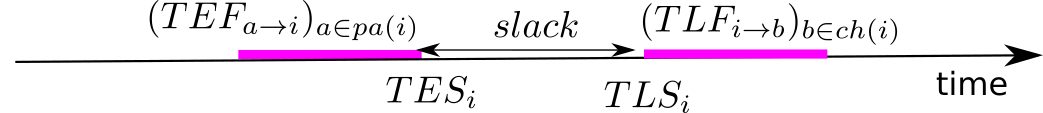
\includegraphics[width=6in]{pert/pert.png}
\caption{
$TES_i$ 
defined from info received
from parents of  $i$
and  $TLS_i$
defined from info received 
from children of $i$.} 
\label{fig-pert-t-interval}
\end{figure}

\section{Example}
To illustrate PERT analysis, we end 
with an example. We present the 
example
in the form of an exercise question and then
provide the answer. This example
comes from Ref.\cite{ibook},
except for part \ref{q-pert-bnets} 
about bnets, which is our own.

{\bf Question:}
For the PERT diagram of Fig.\ref{fig-pert-diag},
calculate the following:


\begin{enumerate}[(a)]
\item\label{q-times} Interval $[TES_i, TLS_i]$
for all $i$.
\item\label{q-critical}A critical path
for this PERT diagram.
\item\label{q-mean-variance-d} The
mean and variance of the total
duration of the critical path.
\item\label{q-prob} The probability that
the total duration will be 225 days or less.
\item\label{q-pert-bnets} A bnet interpretation
of this problem.
\end{enumerate}
\begin{description}

\item[Answer to \ref{q-times}]
$[TES_i, TLS_i]$
are given by Fig.\ref{fig-pert-times}.

\begin{figure}[h!]
\centering
$$\xymatrix{
&&\rvE_3\ar[r]^{40 (0.25)}
&\rvE_6\ar[drr]^{10 (1.00)}
\\
\rvE_1\ar[r]^{50 (2.56)}
&\rvE_2\ar[ru]^{20 (1.00)}
\ar[rd]_{60 (0.44)}
\ar[r]^{20 (0.25)}
&\rvE_4\ar[r]^{60 (2.56)}
&\rvE_7\ar[rd]^{40 (1.31) }
&&\rvE_9\ar[r]^{30 (1.00)}
&\rvE_{10}
\\
&&\rvE_5\ar[ru]^{30 (1.78)}
\ar[rr]_{20 (1.00)}
&&\rvE_8\ar[ru]_{10 (0.64)}
}$$
\caption{Example of a PERT
diagram. The numbers attached to
the arrows are the duration times
 $D_{i\rarrow j}$ in days
followed by, enclosed
in parentheses,
the variance $V_{i\rarrow j}$
of that duration.
The info given
in this PERT diagram
was derived
from a DT table in Ref.\cite{ibook}. The
info in this PERT
diagram 
is sufficient
for calculating
$TES_i$ and $TLS_i$
for each node $i$.
The results of that calculation 
are given in Fig.\ref{fig-pert-times}.
}
\label{fig-pert-diag}
\end{figure}



\begin{figure}[h!]
\centering
$$
\begin{array}{c}
\xymatrix{
&&\rvE_3\ar[r]^{40}70
&\rvE_6\ar[drr]^{10}110
\\
\rvE_1\ar@[red][r]^{50}0
&\rvE_2\ar[ru]^{20}\ar@[red][rd]_{60}\ar[r]^{20}50
&\rvE_4\ar[r]^{60}70
&\rvE_7\ar@[red][rd]^{40}140
&&\rvE_9\ar@[red][r]^{30}190
&\rvE_{10}220
\\
&&\rvE_5\ar@[red][ru]^{30}\ar[rr]_{20}110
&&\rvE_8\ar@[red][ru]_{10}180
}
\\
TES_i \text{ (given after the node name) for node $\rvE_i$ for all $i$}
\\
\\
\xymatrix{
&&\rvE_3\ar[r]^{40}140
&\rvE_6\ar[drr]^{10}180
\\
\rvE_1\ar@[red][r]^{50}0
&\rvE_2\ar[ru]^{20}\ar@[red][rd]_{60}\ar[r]^{20}50
&\rvE_4\ar[r]^{60}80
&\rvE_7\ar@[red][rd]^{40}140
&&\rvE_9\ar@[red][r]^{30}190
&\rvE_{10}220
\\
&&\rvE_5\ar@[red][ru]^{30}\ar[rr]_{20}110
&&\rvE_8\ar@[red][ru]_{10}180
}
\\
TLS_i \text{ (given after the node name) for node $\rvE_i$ for all $i$}
\end{array}
$$
\caption{Results of calculating
$TES_i$  for all $i$ via a forward
pass, followed by calculating
$TLS_i$ for all $i$
via a backward pass.
Critical path indicated in red.}
\label{fig-pert-times}
\end{figure}

\item[Answer to \ref{q-critical}]
The critical path is given 
in red in Fig.\ref{fig-pert-times}.
Note that this path does indeed
have zero slack at each node it
visits and the union of
its neighborhood and 
the path itself encompasses all nodes.
\item[Answer to \ref{q-mean-variance-d}]

The mean
and variance of
the total duration
are calculated in Table \ref{tab-duration}.

% Please add the following required packages to your document preamble:
% \usepackage[table,xcdraw]{xcolor}
% If you use beamer only pass "xcolor=table" option, i.e., \documentclass[xcolor=table]{beamer}
\begin{table}[]
\centering
\begin{tabular}{|l|l|l|}
\hline
\rowcolor[HTML]{FFFFC7} 
\begin{tabular}[c]{@{}l@{}}edge\\ $i\rarrow j$\end{tabular} & \begin{tabular}[c]{@{}l@{}}duration\\ $D_{i\rarrow j}$\end{tabular} & \begin{tabular}[c]{@{}l@{}}variance\\ $V_{i\rarrow j}$\end{tabular} \\ \hline
A ($1\rarrow 2$) & 50 & 2.56 \\ \hline
D ($2\rarrow 5$) & 60 & 0.44 \\ \hline
G ($5\rarrow 7$) & 30 & 1.78 \\ \hline
J ($7\rarrow 8$) & 40 & 1.31 \\ \hline
K ($8\rarrow 9$) & 10 & 0.64 \\ \hline
L ($9\rarrow 10$) & 30 & 1.00 \\ \hline
\rowcolor[HTML]{FFFFC7} 
Total & 220 & 7.73 \\ \hline
\end{tabular}
\caption{Calculation of mean and variance of total duration along critical path.}
\label{tab-duration}
\end{table}

\item[Answer to \ref{q-prob}]

\beqa
P(\rvx<225)&=&P\left[\frac{\rvx-\mu}
{\sigma}\leq 
\frac{225-220}{\sqrt{7.73}}\right]
\\
&=&
P[\rvz\leq1.80]
\\
&=&0.9641
\eeqa


\item[Answer to \ref{q-pert-bnets}]
Define 2 bnets.
\begin{enumerate}
\item
The first PERT bnet is for calculating $TES_i$
for all $i$
and is given by Fig.\ref{fig-pert-bnet-tes}.

\begin{figure}[h!]
\centering
$$\xymatrix{
&&\ul{TES}_3\ar[r]
&\ul{TES}_6\ar[drr]
\\
\ul{TES}_1\ar[r]
&\ul{TES}_2\ar[ru]\ar[rd]\ar[r]
&\ul{TES}_4\ar[r]
&\ul{TES}_7\ar[rd]
&&\ul{TES}_9\ar[r]
&\ul{TES}_{10}
\\
&&\ul{TES}_5\ar[ru]\ar[rr]
&&\ul{TES}_8\ar[ru]
}$$
\caption{bnet for $TES_i$
calculation.}
\label{fig-pert-bnet-tes}
\end{figure}

The TPMs,
printed in blue,
for the bnet Fig.\ref{fig-pert-bnet-tes},
are as follows (this equation
is to be evaluated recursively
by a  forward pass through the
bnet):

\beq\color{blue}
P(TES_i| (TES_a)_{a\in pa(i)})=
\delta(TES_i, 
\max_{a\in pa(i)}
(TES_a + D_{a\rarrow i}))
\eeq

\item
The second PERT bnet is for
calculating $TLS_i$ for all $i$
and is given by Fig.\ref{fig-pert-bnet-tls}.
Note
that the directions
of all the arrows in
the PERT diagram
Fig.\ref{fig-pert-diag} have
been reversed so
Fig.\ref{fig-pert-bnet-tls}
is a time reversed graph.



\begin{figure}[h!]
\centering
$$\xymatrix{
&&\ul{TLS}_3\ar[ld]
&\ul{TLS}_6\ar[l]
\\
\ul{TLS}_1
&\ul{TLS}_2\ar[l]
&\ul{TLS}_4\ar[l]
&\ul{TLS}_7\ar[l]\ar[ld]
&&\ul{TLS}_9\ar[ld]\ar[llu]
&\ul{TLS}_{10}\ar[l]
\\
&&\ul{TLS}_5\ar[lu]
&&\ul{TLS}_8\ar[lu]\ar[ll]
}$$
\caption{bnet for $TLS_i$
calculation.}
\label{fig-pert-bnet-tls}
\end{figure}



The TPMs,
printed in blue,
for the bnet Fig.\ref{fig-pert-bnet-tls},
are as follows (this equation
is to be evaluate recursively
by a  backward pass through the
bnet):

\beq\color{blue}
P(TLS_i| (TLS_b)_{b\in pa(i)})=
\delta(TLS_i, 
\min_{b\in pa(i)}
(TLS_b - D^T_{b\rarrow i}))
\;,
\eeq
where $D^T_{i\rarrow j}= D_{j\rarrow i}$.
\end{enumerate}
\end{description}
 








